\documentclass{article}%
\usepackage[T1]{fontenc}%
\usepackage[utf8]{inputenc}%
\usepackage{lmodern}%
\usepackage{textcomp}%
\usepackage{lastpage}%
\usepackage[head=40pt,margin=0.5in,bottom=0.6in]{geometry}%
\usepackage{graphicx}%
%
\title{\textbf{Guanipa tras ser liberado: Nos golpearon sin ninguna razón}}%
\author{El Nacional Web}%
\date{29/09/2018}%
%
\begin{document}%
\normalsize%
\maketitle%
\textbf{URL: }%
http://www.el{-}nacional.com/noticias/oposicion/guanipa{-}tras{-}ser{-}liberado{-}nos{-}golpearon{-}sin{-}ninguna{-}razon\_253714\newline%
%
\textbf{Periodico: }%
EN, %
ID: %
253714, %
Seccion: %
Oposición\newline%
%
\textbf{Palabras Claves: }%
Zulia, Gobierno\newline%
%
\textbf{Derecho: }%
1.2, %
Otros Derechos: %
1.3, %
Sub Derechos: %
1.2.1, 1.3.2\newline%
%
\textbf{EP: }%
NO\newline%
\newline%
%
\textbf{\textit{El dirigente de la tolda amarilla detalló que los funcionarios no estaban uniformados~}}%
\newline%
\newline%
%
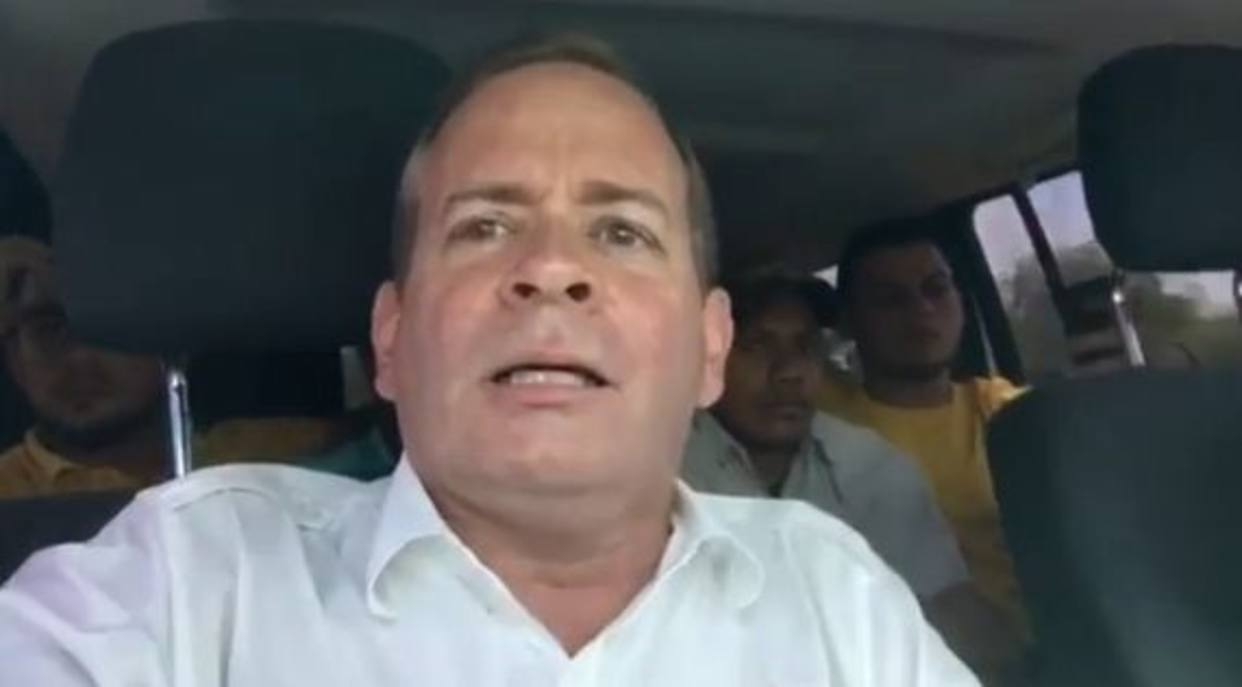
\includegraphics[width=300px]{45.jpg}%
\newline%
%
Juan Pablo Guanipa, dirigente de Primero Justicia,~ aseguró que los sujetos que lo~abordaron se lo llevaron detenido sin ninguna razón.%
\newline%
%
"Nos golpearon,~nos llevaron presos sin ninguna razón. Los funcionarios no portaban~uniforme, estaban de civiles y armados hasta los dientes", explicó en rueda de prensa.%
\newline%
%
Agregó que:~"Los funcionarios nos dijeron; 'ustedes creen que van a hacer una actividad política en San Francisco y van a salir ilesos'".%
\newline%
%
Guanipa detalló que se encontraba haciendo un recorrido~por el municipio San Francisco cuando fue interceptado por varias camionetas con sujetos que, posteriormente, lo agredieron.%
\newline%
%
"Venezuela tiene todo para salir hacia~adelante. Este tipo de acciones no nos van a amedrentar. A todo el pueblo les digo que tenemos derechos de ejercer mecanismos~~de presión", indicó.%
\newline%
%
\end{document}